\documentclass[letterpaper]{article}
\usepackage{natbib,alifexi}
\usepackage[utf8]{inputenc}
\usepackage[francais]{babel}
\usepackage{hyperref}
\usepackage{tikz}
\usetikzlibrary{tikzmark,arrows.meta}
\usepackage{amsmath}
\usepackage{amssymb}
\usepackage{graphicx}


\addto\captionsfrench{%
  \renewcommand{\tablename}{Fig.}%
}


\title{Mini-Tor : Le réseau Tor démystifié}
\author {Nathan Liccardo \\ \mbox{} \\ nathan.liccardo@ulb.ac.be}


\begin{document}
\maketitle

\begin{abstract}
Dans le cadre de mon mémoire de fin de bachelier, j'ai décidé d'aborder le réseau d'anonymisation de connexions et communications Tor. Afin de réaliser mon travail, il m'a été demandé, dans un premier temps, de comprendre l'architecture de ce système afin de pouvoir, dans un second temps, implémenter le système de façon schématique et moins complexe que celui du réseau Tor (original). On retrouvera donc dans l'ensemble de ce document à la fois la partie théorique de mon travail reprenant les concepts sur lesquels reposent le réseau mais également les détails de mon implémentation permettant de retrouver et d'illustrer ces concepts. Je tiens à remercier Monsieur François Gérard pour son aide précieuse lors de la rédaction et l'implémentation de ce travail. 
\end{abstract}


\section{Introduction}
Selon la page officielle du projet Tor \cite{ref1}, ce dernier a pour objectif principal d'améliorer la vie privée des utilisateurs ainsi que l'anonymat de ces derniers sur internet. Tor serait également un outil efficace contre la censure permettant aux personnes utilisant le réseau de pouvoir avoir accès aux contenus bloqués par certaines formes de régimes autoritaires. Tout au long de ce document, je détaillerai les techniques informatiques utilisées afin de pouvoir créer un réseau tel que Tor. Afin d'expliciter le mieux possible les différents concepts abordés, un réseau Tor simplifié a également été développé. Ce développement est repris en annexe du présent document. Tor utilise au sein de son réseau différentes techniques de chiffrement et déchiffrement des messages. L'ensemble des termes directement liés à la sécurité ainsi que les techniques de chiffrement seront donc détaillés dans un premier temps afin de pouvoir ensuite expliciter le fonctionnement de Tor. Mon intérêt pour le réseau Tor est lié aux techniques informatiques évoluées (que nous verrons dans la suite du document) mais également aux aspects socio-politiques. Tor reste, à l'heure actuelle, un outil majeur pour la défense de la liberté d'expression dans certains pays. \\

Avant d'aborder le coeur du sujet et les différents aspects techniques de Tor, il est intéressant de se pencher un instant sur l'histoire de ce réseau. Si l'on se base sur la page officielle des membres du réseau Tor \cite{ref2}, on trouve deux noms incontournables à savoir Roger Dingledine et Nick Mathewson. Ces deux informaticiens (aujourd'hui Président et Vice-Président du projet) sont à l'origine du réseau. Il est important de noter que le routage en oignon, à savoir l'envoi de messages enveloppés sous plusieurs couches distinctes, a été développé dans les années 1990 mais que le réseau, basé sur cette technique, n'a été rendu disponnible qu'en 2002 dans sa version alpha \cite{ref4} et c'est en 2004 que \og The Second-Generation Onion Router \fg est présenté. Enfin, c'est en 2006 que \og The Tor Project\fg a été créé \cite{ref3}. Ce dernier a pour objectif de maintenir et mettre à jour continuellement le réseau \cite{ref1}.  \\

Si l'on se réfère une fois de plus au site officiel de Tor \cite{ref1}, on constate que l'anonymat \footnote{Anonymat : Etat de quelque chose, quelqu'un qui est anonyme à savoir, dont l'auteur ou le nom est inconnu} total ne peut être atteint. Le réseau Tor représente donc un outil mis à disposition de manière libre et permettant aux utilisateurs de sécuriser \footnote{Sécuriser : Rendre quelque chose plus sûr, fiabiliser} le transport de leurs données d'un point A à un point B. Tor ne permet en aucun cas d'assurer une sécurisation de l'utilisateur mais bel et bien d'anonymiser les requêtes effectuées par ce dernier. Afin d'assurer l'anonymat de l'utilisateur, le groupe Tor Project conseille d'utiliser ce que l'on appelle un \og protocol-specific support software \fg qui permettra de masquer les données permettant de l'identifier. The Tor Project a conçu un navigateur web permettant d'utiliser Tor tout en masquant et bloquant les possibilités d'identification de l'utilisateur. \\

Le corps de ce document sera découpé en trois grandes parties. La première abordera les notions de chiffrements des données. Cette partie permettra de comprendre, dans le détail, la façon dont fonctionne la modification d'apparence des informations. Nous poursuivrons ensuite avec les notions de routage en oignon (seconde section) pour enfin finir avec l'explication du système Tor (troisième section).

\section{Chiffrement}
La question de la modification des données au sein du réseau Tor est un élément important si l'on souhaite en comprendre correctement le fonctionnement. Partant de la représentation d'un message, le chiffrement permet d'obtenir une représentation différente et non compréhensible du message originel. Dans les versions les plus anciennes, les méthodes de chiffrements nécessitaient un accord préalable entre les correspondants afin de pouvoir comprendre les messages échangés. Cette méthode pouvait être extrêmement complexe à mettre en place si les correspondants n'avaient pas de moyens aisés et sécurisés pour échanger les informations nécessaires. C'est pour cette raison que des techniques plus évoluées ont été mises en place. Avec ces nouvelles méthodes, l'objectif sera de simplifier l'échange des informations sans risquer d'affaiblir la méthode de chiffrement. Il existe, à l'heure actuelle, deux techniques permettant de chiffrer des données à savoir : le chiffrement asymétrique et symétrique. Dans la suite de ce document, lorsque nous parlerons de chiffrement des données, cela reviendra à appliquer un algorithme appartenant à l'une de ces deux familles sur un paquet de données. Voici une illustration permettant de schématiser de manière simple le fonctionnement d'une fonction de chiffrement (que l'on utilise la technique symétrique ou asymétrique) : \\ 

\begin{tikzpicture}
\draw (-1.5,-0.25) node{Données} ;
\draw (-1.5,-0.65) node{(non chiffrées)} ;
\draw[->] (-0.4,-0.5) -- (0.15,-0.5);
\pgfmathsetmacro{\cubex}{2}
\pgfmathsetmacro{\cubey}{1}
\pgfmathsetmacro{\cubez}{1}
\draw[black] (2.2,0,0) -- ++(-\cubex,0,0) -- ++(0,-\cubey,0) -- ++(\cubex,0,0) -- cycle;
\draw[black] (2.2,0,0) -- ++(0,0,-\cubez) -- ++(0,-\cubey,0) -- ++(0,0,\cubez) -- cycle;
\draw[black] (2.2,0,0) -- ++(-\cubex,0,0) -- ++(0,0,-\cubez) -- ++(\cubex,0,0) -- cycle;
\draw (1.2,-0.47) node{Algorithme};
\draw[->] (2.65,-0.5) -- (3.35,-0.5);
\draw (4.1,-0.25) node{Données};
\draw(4.1,-0.65) node{(chiffrées)};
\end{tikzpicture} \\

Dans cette section, je commencerai par détailler le principe du chiffrement asymétrique (RSA \cite{ref6}) afin de développer ensuite le chiffrement symétrique (AES \cite{ref8}). Les algorithmes mathématiques appliqués sur les données afin d'obtenir une valeur de sortie différente se basent sur l'utilisation de clés de chiffrement. L'utilisation d'algorithmes symétriques ou asymétriques définira la manière dont on effectuera l'échange des clés permettant le chiffrement et déchiffrement des messages. Une fois échangées, on utilisera ces clés afin de pouvoir appliquer une transformation des données. Les clés utilisées par les algorithmes peuvent être de types différents (câblage électrique, chaine de caractères, chaine binaire...). Nous utiliserons, dans le cadre de ce rapport, des clés composées de différents caractères pouvant être des chiffres ou des lettres.
\subsection{Asymétrique}
Le chiffrement asymétrique est le premier type de chiffrement que nous aborderons. Il est défini par l'utilisation de deux clés différentes dont l'une permet de chiffrer les données et l'autre de les déchiffrer \footnote{Action de déchiffrer à savoir lire ou comprendre un texte écrit peu lisible ou codé.}. Les algorithmes appartenant à cette famille se basent sur les fonctions à sens unique.
\subsubsection{Fonctions à sens unique} Soit $n \in \mathbb{N} $, on pose les ensembles finis suivants  $ A_n = \{ 1,2,...,n \} $ et $B_n$. La fonction : 
\begin{center}
$f_n : A_n \rightarrow B_n$
\end{center}
est définie comme à sens unique si : \vspace{0.03cm}
\begin{itemize}
\item[-] Il est facile de calculer $f_n(x)$ pour un $n$ très grand ($x \in A_n$). $\rightarrow$ $f_n$ facile à calculer .
\item[-] Il est difficile pour $y \in f_n(A_n)$ de trouver un $x$ tel que $f(x) = y$. $\rightarrow$ $f_n$ difficile à inverser. \\
\end{itemize}
On comprend alors pourquoi les algorithmes de chiffrement asymétriques disposent de deux clés (publique et privée) et pourquoi l'action de déchiffrement des données est considérée comme extrêmement lente. Malgré la lenteur apparente des algorithmes de ce type, ils restent néanmoins largement utilisés lorsque la distribution de la clé doit être effectuée auprès d'un grand nombre de personnes (ex : connexions internet à un serveur sécurisé).
\subsubsection{RSA}
 L'algorithme le plus connu des systèmes asymétriques est connu sous le nom de RSA \cite{ref6}. Il a été développé en 1978 par Ron Rivest, Adi Shamir et Leonard Adleman \cite{ref7}. Ce dernier porte comme nom les initiales de ses trois créateurs et se définit par l'utilisation de deux clés différentes pour le chiffrement et le déchiffrement des données. Afin de pouvoir utiliser cet algorithme, il faut commencer par choisir deux nombres premiers $p$ et $q$. A partir de ces deux nombres, on calcule alors $N = p*q$ pour enfin obtenir : \vspace{-0.2cm}
\begin{equation}
\varphi(N) = (p-1)*(q-1)\vspace{-0.1cm}
\end{equation}
On choisit ensuite un entier $e$ pour lequel les deux équations suivantes doivent être respectées : \vspace{-0.2cm}
\begin{equation}
1 < e < \varphi(N)
\end{equation}\vspace{-0.5cm}
\begin{equation}
pgcd(e,\varphi(N)) = 1)
\end{equation}
Les valeur de $e$ et de $\varphi(N)$ sont alors utilisées pour calculer la valeur de $d$ suivant la définition :\vspace{-0.2cm}
\begin{equation}
e*d \equiv 1 \mod \varphi(N) \vspace{-0.1cm}
\end{equation}
On peut alors, à partir des valeurs obtenues, créer une clé privée ($d_K(c)$) ainsi qu'une clé publique ($e_K(m)$) que l'on utilisera par la suite pour chiffrer et déchiffrer nos données : 
\begin{center}
$d_K(c) := c^d \mod N$  \vspace{0.2cm} \\
$e_K(m) := m^e \mod N$
\end{center}
RSA est fondé sur l'utilisation de grands nombres ainsi que la difficulté de factoriser ces derniers \cite{ref6}. Il n'existe cependant à l'heure actuelle aucune preuve mathématique permettant d'affirmer l'équivalence entre le problème de factorisation et le déchiffrement aisé. On se base donc principalement sur des intuitions mathématiques. L'utilisation de grands nombres signifie utiliser des clés d'au moins 1024 bits. \\
\begin{tikzpicture}
\draw (-3.15,-0.25) node{Données} ;
\draw (-3.15,-0.65) node{(non chiffrées)} ;
\pgfmathsetmacro{\cubex}{2.3}
\pgfmathsetmacro{\cubey}{1}
\pgfmathsetmacro{\cubez}{1}
\draw[black] (-2,0,0) -- ++(-\cubex,0,0) -- ++(0,-\cubey,0) -- ++(\cubex,0,0) -- cycle;
\draw[black] (-2,0,0) -- ++(0,0,-\cubez) -- ++(0,-\cubey,0) -- ++(0,0,\cubez) -- cycle;
\draw[black] (-2,0,0) -- ++(-\cubex,0,0) -- ++(0,0,-\cubez) -- ++(\cubex,0,0) -- cycle;
\draw (-0.25,-0.47) node{RSA};
\draw (2.2,-0.25) node{Données};
\draw (2.2,-0.65) node{(chiffrées)};
pgfmathsetmacro{\cubex}{2}
\pgfmathsetmacro{\cubey}{1}
\pgfmathsetmacro{\cubez}{1}
\draw[black] (3.3,0,0) -- ++(-\cubex,0,0) -- ++(0,-\cubey,0) -- ++(\cubex,0,0) -- cycle;
\draw[black] (3.3,0,0) -- ++(0,0,-\cubez) -- ++(0,-\cubey,0) -- ++(0,0,\cubez) -- cycle;
\draw[black] (3.3,0,0) -- ++(-\cubex,0,0) -- ++(0,0,-\cubez) -- ++(\cubex,0,0) -- cycle;
\draw[red, thick,rounded corners=8pt,->] (-2,0)--(-0.5,0.5) node[yshift=0.2cm]{$e_K(m)$} --(1,0);
\draw[red, thick,rounded corners=8pt,<-] (-2,-1)--(-0.5,-1.5) node[yshift=-0.2cm]{$d_K(c)$} --(1,-1);
\end{tikzpicture} \newline
Il est à noter que les fonctions de chiffrement et déchiffrement appliquées sont commutatives. 

\subsection{Symétrique}
Abordons à présent le second type de chiffrement à savoir symétrique. Dans ce cas, les clés de chiffrement et déchiffrement correspondent a une et une seule clé. Il n'est donc plus question de rendre publique l'une des deux clés mais bien de communiquer la clé secrète de manière sécurisée. Le chiffrement symétrique se divise également en deux grandes catégories à savoir le chiffrement par bloc (que nous verrons par la suite) et le chiffrement par flot \cite{ref9}. Voyons premièrement la différence qui existe par rapport au chiffrement asymétrique. La méthode symétrique tire son avantage de par sa rapidité de déchiffrage des données. Elle s'appuie sur des fonctions inversibles et efficaces \cite{ref9}. Un algorithme de chiffrement symétrique se définit comme la transformation d'un message M avec une clé secrète K. Le résultat est un message chiffré C :  \\

\begin{tikzpicture}
\draw (-3.5,-0.5) node{$M = \{ 0,1 \}^n$} ;
\draw[->] (-2.5,-0.5)--(-1.6,-0.5);
\pgfmathsetmacro{\cubex}{2.3}
\pgfmathsetmacro{\cubey}{1}
\pgfmathsetmacro{\cubez}{0}
\draw[black] (0.8,0,0) -- ++(-\cubex,0,0) -- ++(0,-\cubey,0) -- ++(\cubex,0,0) -- cycle;
\draw[black] (0.8,0,0) -- ++(0,0,-\cubez) -- ++(0,-\cubey,0) -- ++(0,0,\cubez) -- cycle;
\draw[black] (0.8,0,0) -- ++(-\cubex,0,0) -- ++(0,0,-\cubez) -- ++(\cubex,0,0) -- cycle;
\draw (-0.33,-0.5) node{Chiffrement};
\draw[->] (0.9,-0.5)--(1.55,-0.5);
\draw[->] (-0.25,-1.7)--(-0.25,-1.1);
\draw (2.5,-0.5) node{$C = \{ 0,1 \}^n$};
\draw (-0.35,-2) node{$K = \{ 0,1 \}^k$};
\end{tikzpicture}
Les algorithmes à chiffrement symétrique fonctionnent généralement par bloc ce qui implique que le message est alors traité par morceaux de données de tailles équivalentes \footnote{On découpe le message en blocs de tailles équivalentes}. La technique consiste à effectuer un premier traitement durant lequel on découpe le message afin d'obtenir une succession de blocs pouvant être traités. Comme mentionné dans le cours de Monsieur Ferradi \cite{ref10}, il existe deux principes fondamentaux qui sont utilisés dans le chiffrement symétrique par blocs à savoir : la confusion et la diffusion.
\subsubsection{Confusion} Masquer toute relation linéaire entre le chiffré et le message en clair. \vspace{-0.2cm}
\subsubsection{Diffusion} Cacher la redondance en répartissant l'influence d'un bit de clé sur tout le chiffré. \vspace{0.3cm}

\noindent Ces deux techniques seront donc appliquées sur chaque bloc pris indépendamment l'un de l'autre. Pour finir, remarquons également que les fonctions de chiffrement symétrique sont également inversibles. Il en découle que ces fonctions sont bijectives. Afin d'illustrer au mieux le fonctionnement d'un chiffrement symétrique, nous utiliserons dans ce rapport le système AES (Advanced Encryption Security).

\subsubsection{EAS} Il a été développé dans les années 2000 et est basé sur un algorithme itératif. Le nombre d'exécutions sera directement lié à la taille de la clé utilisée à savoir 128 ou 256 bits (10 ou 14 itérations). Pour chaque itération, l'algorithme effectuera une action de confusion (substitution non-linéaire) suivie d'une diffusion (permutation linéaire). De manière exacte, AES commence par placer l'ensemble des données (sous forme d'octets) dans une matrice 4*4 (128 bits maximum) :
\begin{center}
	$\begin{bmatrix}
	a_{11} & a_{12} & a_{13} & a_{14} \\
	a_{21} & a_{22} & a_{23} & a_{24} \\
	a_{31} & a_{32} & a_{33} & a_{34} \\
	a_{41} & a_{42} & a_{43} & a_{44} \\
	\end{bmatrix}$
\end{center}
Il effectue ensuite l'opération XOR \footnote{Ou exclusif} pour chaque byte avec le byte correspondant dans la clé fournie (128 bits) à savoir : 
\begin{center}
$A_{i,j} \oplus K_{i,j} = B_{i,j}$
\end{center}
AES construit ensuite une transformation non-linéaire (à savoir la confusion) couramment appelée \og SubBytes \fg : 
\begin{center}
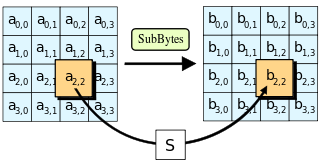
\includegraphics[scale=0.7]{imageADD.png}\\
\end{center}
Une fois la transformation non-linéaire obtenue, il faut appliquer la transformation linéaire de la matrice résultante. Il s'agit alors de la diffusion citée précédemment. AES applique une transformation circulaire vers la gauche : 
\begin{center}
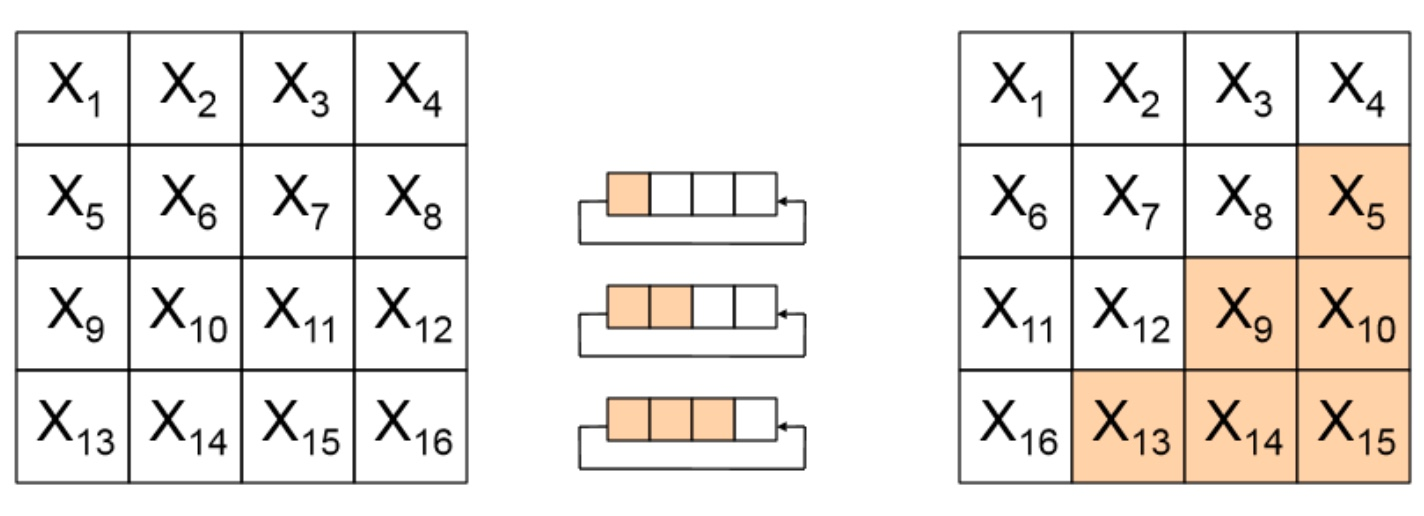
\includegraphics[scale=0.165]{imageStep4}\\
\end{center}
Pour finir, l'algorithme applique un mélange des colonnes de la matrice finale : 
\begin{center}
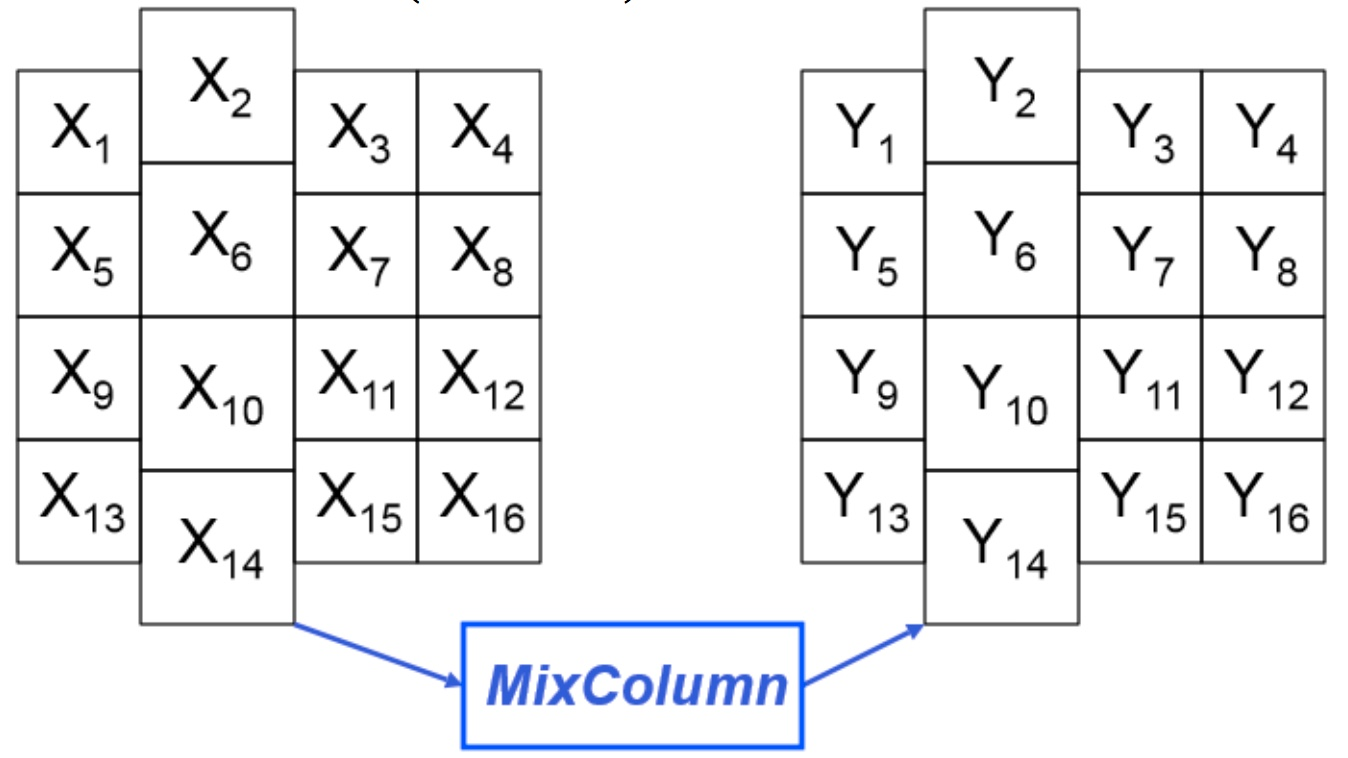
\includegraphics[scale=0.17]{image4}\\
\end{center}
On a maintenant le détail de l'ensemble des étapes à effectuer afin d'obtenir un message chiffré via le système AES.

\subsection{Echange de clés}
Après avoir détaillé les deux méthodes existantes pour chiffrer et déchiffrer des messages, il en résulte que chacune a ses avantages et ses inconvénients. L'objectif serait de combiner la rapidité d'exécution de la méthode symétrique avec les avantages de la clé publique dans le cas des systèmes asymétriques. Pour ce faire, une des techniques les plus répandues repose sur l'échange de clés symétriques au travers d'un chiffrement asymétrique. Prenons, à titre d'exemple, le cas d'un échange client-serveur. Le client va alors récupérer la clé publique du serveur afin de pouvoir appliquer un chiffrement asymétrique (RSA) sur une clé de chiffrement symétrique (AES) qu'il aura lui-même généré. Il va alors initier une communication avec le serveur qui permettra d'échanger la clé symétrique. Une fois l'échange terminé, les deux entités (client/serveur) pourront alors communiquer à l'aide d'un système efficace (rapide). On peut également, lorsque l'on souhaite augmenter la sécurité, renouveler la clé symétrique après un certains temps ou un certain nombre d'échanges. Afin d'être le plus complet possible, il est à noter qu'il existe d'autres types d'échanges de clés. L'un des plus connus (que nous ne détaillerons pas ici) est l'échange de clés Diffie-Hellman. Il est intéressant de souligner que cette méthode n'utilise en aucun cas le chiffrement asymétrique. Cet aspect permet donc une plus grande rapidité.

\section{Problème d'anonymat}
L'anonymisation des données échangées au travers du réseau internet est une des principales problématiques de ces dix dernières années. Il est en effet de plus en plus courant d'entendre, via les différents médias, diverses histoires d'écoutes informatiques. Ces dernières reposent généralement sur le lien existant entre deux entités communicantes. Si nous prenons par exemple le cas d'un échange client-serveur, on pourrait imaginer d'intercepter les échanges effectués par l'ensemble des utilisateurs se connectant à ce serveur. Cela mettrait alors en péril l'anonymat des individus. L'analyse du traffic pourrait, dans un premier temps, porter préjudice à la vie privée mais également, dans un second temps, porter atteinte à la liberté d'autrui. Si l'on prend l'exemple d'un régime autoritaire souhaitant restreindre l'accès à certains sites internet, il va alors, en analysant les données transitant sur le réseau des utilisateurs, bloquer les différents accès aux sites non désirés. On aperçoit bel et bien l'apparition d'une forme de censure. L'une des réponses apportées au problème d'anonymat est le routage en oignon. Ce procédé, qui sera détaillé dans la suite de la section, est également le fondement même du réseau Tor. Il sera donc primordial d'en comprendre les fondements.

\subsection{Routage en oignon}
Le routage en oignon (Onion routing) a été développé par un mathématicien et deux informaticiens du nom de Paul Syverson, Macheal G Reed et David Goldschlag dans les bureaux de la marine américaine. l'objectif de ces trois hommes était d'empêcher les écoutes sur les communications de la marine des Etats-Unis \cite{ref11}. Pour comprendre correctement le fonctionnement de l'onion routing, revenons un instant sur l'objectif de celui-ci. Lorsqu'une connexion est établie entre deux entités, on s'aperçoit qu'elle peut être interceptée et écoutée. Dans un premier temps, partons de l'idée que le chiffrement des données serait une solution à notre problème. Malheureusement, le fait d'appliquer un chiffrement au message ne rend pas ce dernier impossible à suivre. La solution apportée par le routage en oignon sera alors d'insérer un certain nombre de passerelles (appelées noeuds) entre les deux entités communicantes. Pour chaque message transitant dans le réseau, on appliquera un nombre de couches $n$ correspondant au nombre de noeuds intermédiaires empruntés par le message. On procédera alors à ce que l'on appelle une encapsulation des messages.
\begin{center}
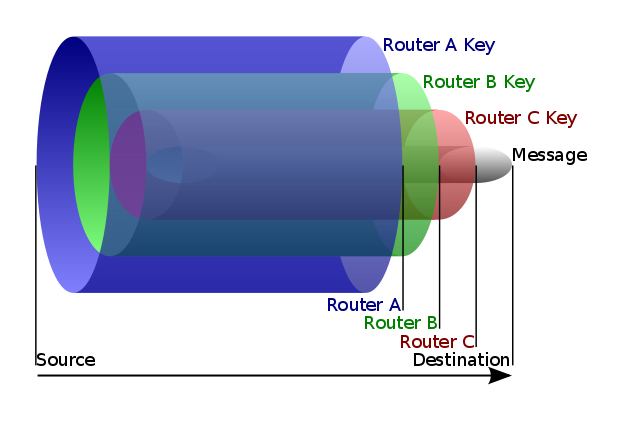
\includegraphics[scale=0.3]{imageOnionRouting.png}
\end{center}
\subsubsection{Encapsulation de messages}
Les messages utilisés seront formatés sous la forme d'oignons. L'idée est d'imbriquer les messages les uns dans les autres sur le modèle des poupées russes. Pour obtenir une illustration concrète, basons nous sur le message suivant : 	
\begin{table}[!htbp]
\centering
\begin{tabular}{|l|l|l|}
\hline
Noeud & Clé & Message \\ \hline
\end{tabular}
\end{table}
\newline
Une fois que nous avons établi une structure du message, il nous est possible de construire un oignon pouvant transiter au sein du réseau. L'oignon sera alors construit de la façon suivante : \\
\begin{table}[!htbp]
\centering
\begin{tabular}{|l|l|l|}
\hline
Noeud & Clé & Message \\ \hline
\end{tabular}
\begin{tikzpicture}[overlay]
 \draw[black, line width=1pt] (-2.065,0.09) ellipse (3cm and 0.55cm);
\end{tikzpicture} 
\end{table}
\begin{table}[!htbp]
\centering
\begin{tabular}{|l|l|l|}
\hline
Noeud & Clé & Message \\ \hline
\end{tabular}
\begin{tikzpicture}[overlay]
 \draw[black, line width=1pt] (-2.065,0.09) ellipse (3cm and 0.55cm);
\end{tikzpicture} 
\end{table}
\begin{table}[!htbp]
\centering
\begin{tabular}{|l|l|l|}
\hline
Noeud & Clé & Message \\ \hline
\end{tabular}
\begin{tikzpicture}[overlay]
 \draw[black, line width=1pt] (-2.065,0.09) ellipse (3cm and 0.55cm);
\end{tikzpicture} 
\end{table}

\begin{table}[!htbp]
\centering
%\hskip-.1cm
\begin{tabular}{|l|l|l|}
\hline
Noeud & Clé & Message \\ \hline
\end{tabular}
\end{table}

\begin{tikzpicture}[overlay]
  \draw[->,rounded corners=8pt] (6.4,4.65)--(7,4.1)--(5.6,3.6);
  \draw[->,rounded corners=8pt] (6.4,3.35)--(7,2.8)--(5.6,2.3);
  \draw[->,rounded corners=8pt] (6.4,2.05)--(7,1.5)--(5.65,1.02);
\end{tikzpicture} 

\noindent Chaque pont intermédiaire sera capable de supprimer une couche du message (de la même façon que l'on pelle un oignon) afin d'en obtenir un nouveau. On constate alors que l'apparence du message diffère après chaque passage par un noeud. Lorsqu'il entre dans un noeud sous un aspect $A$ et qu'il en ressort sous un autre aspect $B$, la mise en relation des deux messages est rendue plus difficile. Cette technique permettra de rendre le suivi du message beaucoup plus complexe. Malgré tout, si l'on se limite à la modification du message, il est tout de même possible de tracer ce dernier. On relèvera par exemple la possibilité de calculer le temps de traitement d'un noeud intermédiaire. Ce procédé permettrait alors de faire correspondre les messages entrant avec ceux sortant du noeud. Pour éviter cela, les noeuds sont en général dotés de minuteurs aléatoires intégrants un temps entre le traitement et la redirection du message

\section{Le réseau Tor}
Tor est une implémentation immédiate du système de routage en oignon détaillé précédemment et est en lien direct avec la problématique d'anonymat. Pour comprendre la manière dont Tor fonctionne, nous en étudierons plusieurs composantes. Il sera dans un premier temps question des clients. Ce sont eux qui souhaitent pouvoir effectuer des requêtes de manière anonyme. Nous détaillerons ensuite les noeuds (passerelles) permettant l'utilisation des messages sous formes d'oignon. Pour finir, nous aborderons brièvement les différents répertoires utilisés afin de récupérer les points de connexions au réseau Tor (Directory Authorities). Cette section s'achèvera par le passage en revue des attaques existantes contre le réseau Tor.

\subsection{Clients}
Les clients souhaitant se connecter et utiliser le réseau Tor auront deux actions à effectuer afin de pouvoir utiliser le réseau; la création d'un chemin et la création de messages. Elles seront réalisées de manière transparente pour l'utilisateur lorsqu'il utilisera par exemple le Tor Web Browser développé par The Tor Project.
\subsubsection{Création d'un chemin} Lorsque le client se connecte au réseau Tor, il effectue en réalité une requête lui permettant de récupérer une liste de noeuds intermédiaires accessibles. Ces différents noeuds seront ensuite utilisés dans le cadre du routage en oignon expliqué précédemment. Le réseau Tor a pris comme convention l'utilisation de trois noeuds intermédiaires. Une fois obtenus, il est donc possible pour le client de créer des messages et de les envoyer sur le réseau.
\subsubsection{Création de messages} Les messages créés par le client seront quant à eux directement liés au circuit obtenu précédemment \footnote{Le circuit est le chemin résultant après avoir choisi trois noeuds aléatoires dans la liste de noeuds accessibles}. Ils disposeront, comme détaillé précédemment, d'une structure sous forme d'oignon. \\
\vspace{2pt}
\begin{table}[!htbp]
\centering
\begin{tabular}{|l|l|l|}
\hline
Noeud & Clé & Message \\ \hline
\end{tabular}
\begin{tikzpicture}[overlay]
 \draw[black, line width=1pt] (-2.065,0.09) ellipse (3cm and 0.55cm);
\end{tikzpicture} 
\end{table}

\begin{table}[!htbp]
\centering
\begin{tabular}{|l|l|l|}
\hline
Noeud & Clé & Message (chiffré) \\ \hline
\end{tabular}
\begin{tikzpicture}[overlay]
 \draw[black, line width=1pt] (-2.65,0.09) ellipse (3cm and 0.55cm);
\end{tikzpicture} 
\end{table}

\begin{table}[!htbp]
\centering
\begin{tabular}{|l|l|l|}
\hline
Noeud & Clé & Message (chiffré) \\ \hline
\end{tabular}
\begin{tikzpicture}[overlay]
 \draw[black, line width=1pt] (-2.65,0.09) ellipse (3cm and 0.55cm);
\end{tikzpicture} 
\end{table}

\begin{table}[!htbp]
\centering
\hskip-.1cm
\begin{tabular}{|l|l|l|}
\hline
Noeud & Clé & Message (chiffré) \\ \hline
\end{tabular}
\end{table}

\begin{tikzpicture}[overlay]
  \draw[->,rounded corners=8pt] (6.4,4.95)--(7,4.4)--(6.2,3.8);
  \draw[->,rounded corners=8pt] (6.4,3.55)--(7,3.1)--(6.2,2.45);
  \draw[->,rounded corners=8pt] (6.4,2.2)--(7,1.8)--(6.2,1.1);
\end{tikzpicture} 

\subsection{Noeuds}
Maintenant que nous avons détaillé les éléments liés à l'utilisateur, il est intéressant d'analyser la manière dont les messages sont traités par les noeuds. Les messages transitant sur le réseau peuvent en effet contenir différents types d'actions \cite{ref14}. On peut par exemple initialiser une nouvelle connexion ou la fermer, faire transiter un message, etc. Nous nous intéresserons principalement à deux fonctionnalités à savoir l'instanciation d'une connexion et le transit d'un message. 
\subsubsection{Ouverture d'un circuit} Lorsqu'un client ouvre son circuit, ce dernier envoi un premier message de création. Dans ce cas, nous utiliserons un système de chiffrement asymétrique permettant l'échange de clés symétriques. On trouvera dans la cellule \og noeud \fg l'adresse de la passerelle suivante et dans la cellule \og clé \fg la clé symétrique correspondant au noeud. 
\subsubsection{Transit de messages} Une fois le circuit initialisé, les messages transitant par le réseau ne doivent plus contenir de clés symétriques étant donné qu'elles ont été échangées précédemment. Chaque noeud est donc considéré comme une plateforme permettant de modifier l'aspect du message en le déchiffrant via sa clé symétrique. \\

\subsection{Directory Authorities} La liste des noeuds accessibles est récupérée auprès de ce que l'on appelle les Directory Authorities \cite{ref1}. Ces derniers sont au nombre de 10 et sont maintenus par l'organisation The Tor Project. Ils représentent également le coeur même du réseau. Une défaillance de ces serveurs entraînerait effectivement l'impossibilité de récupérer de manière correcte les noeuds disponibles. Au vu du nombre restreint de serveurs présents, on retrouve les adresses correspondantes directement écrites dans le code du projet Tor. Voici leurs localisations : \vspace{0.2cm}
\begin{center}
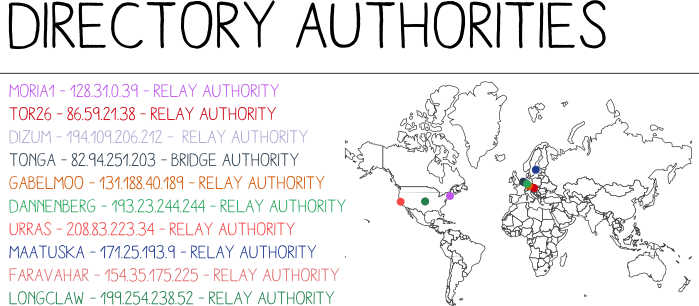
\includegraphics[scale=0.38]{image2} \vspace{0.3cm}
\end{center} 

\subsection{Attaques}
Maintenant que nous avons abordé les trois éléments constituant le réseau ainsi que leurs interactions, il est intéressant d'observer les différents aspects pouvant toutefois rendre les utilisateurs vulnérables. Un certain nombre d'attaques peuvent porter sur ce réseau en mettant soit l'utilisateur soit le réseau en danger \cite{ref14}. Afin de pouvoir détailler de manière exhaustive les différents types d'attaques possibles, nous séparerons ces dernières en trois catégories à savoir : les attaques passives (écoutes), les attaques actives (modifications) et les attaques serveur (sur les Directory Authorities) \cite{ref14}.
\subsubsection{Attaques passives} Ces attaques sont liées à l'écoute de messages ou de trafics. Lorsqu'un individu écoute les connexions établies par un utilisateur, il lui est dans un premier temps impossible de faire correspondre les messages qui sont envoyés par cet utilisateur après le premier noeud. Cela l'empêche alors de connaître les messages transmis. Malheureusement, les messages échangés avec un serveur web gardent généralement une trace de l'utilisateur. Ce sont ces données (contenues au sein des messages échangés) qui vont permettre à l'attaquant de faire correspondre les messages. Il est donc vivement conseillé de supprimer les données concernant l'utilisateur au sein des messages mais également d'utiliser des connexions sécurisées entre le dernier noeud et le serveur afin de ne pas compromettre l'anonymat de l'utilisateur.
\subsubsection{Attaques actives} Les attaques actives, quant à elles, représentent une action réelle de l'attaquant ne se limitant plus à de simples écoutes. Les deux attaques décrites seront directement basées sur l'utilisation des noeuds de sortie. La première consiste à utiliser ces derniers comme protection. En effet, l'ensemble du trafic sortant d'un noeud de sortie lui est attribué. L'administrateur pourrait donc être tenu responsable du trafic illégal passant par son noeud de sortie. La seconde attaque quant à elle repose sur la création de plusieurs noeuds espions. Il faut alors persuader les serveurs qu'il s'agit d'un noeud sécurisé. Dans ce dernier cas, plus l'attaquant arrivera à ajouter des noeuds, plus il sera capable de contrôler le trafic d'un utilisateur.  Il est donc primordial de vérifier la validité des noeuds insérés sur le réseau.
\subsubsection{Attaques des Directory Authorities} Il existe une dernière catégorie d'attaques beaucoup moins répandues étant donné leur niveau de difficulté. Ces dernières portent directement sur les serveurs regroupant la liste des noeuds accessibles. Dans ce type d'attaque, le but est de faire croire aux serveurs qu'un noeud hostile est tout à fait fiable. Lorsque plus de la moitié des serveurs ont contrôlé un noeud, ce noeud est considéré comme valide, si un attaquant parvient à prendre le contrôle de plus de la moitié des serveurs, il sera donc également capable d'insérer autant de noeuds hostiles qu'il souhaite. \\

\noindent Malgré le grand nombre d'attaques existantes, le réseau Tor reste toutefois l'un des réseaux garantissant le plus haut niveau d'anonymat aux utilisateurs.


\section{Implémentation}
Un programme de messagerie a également été implémenté afin de comprendre les techniques utilisées dans le réseau Tor. L'architecture de ce projet reprend l'idée du réseau et permet d'en visualiser les différents concepts. La messagerie a pour le moment été configurée pour deux utilisateurs locaux. Cependant, il est tout à fait possible de changer les adresses de connexion afin de pouvoir l'exécuter sur plusieurs périphériques. Afin de pouvoir utiliser la messagerie, il faut lancer au minimum (et dans l'ordre) un serveur principal permettant de récupérer les informations de connexions, trois noeuds (ou plus) permettant de jouer le rôle de passerelles et, pour finir, deux clients. Il est évident que le projet aurait pu être amélioré ou complexifié. Cependant, il représente une schématisation idéale du réseau et peut être utilisé comme illustration des différents concepts évoqués ci-dessus. Les différents programmes utiles ont été réalisés en Java. Ils peuvent donc être portés sur toute machine disposant de Java. Le choix du langage a été encouragé par l'ensemble de ses possibilités en matière de communications réseau. En effet, Java est un langage offrant un certain nombre de facilités lors de l'échange de messages. Il est évident que d'autres langages auraient pu être tout aussi pertinents. 


\section{Aspects sociaux}
Ma volonté première, lors du choix de ce sujet, était de mettre en avant les différents aspects techniques de Tor. Il est également courant d'entendre parler de ce réseau dans le cadre d'affaires judiciaires. Je trouvais aussi important de relever les aspects politiques et sociaux que Tor pouvait abonder. L'anonymisation des connexions permet effectivement l'accès à divers médias libres et indépendants dans certains pays qui appliquent la censure. Outre les nombreux journalistes utilisant la plateforme, bon nombre de défenseurs des droits humains utilisent également le réseau pour pouvoir communiquer de manière anonyme dans leur pays. Encore à l'heure actuelle, Tor joue un rôle socio-politique majeur dans certaines régions du monde.

\section{Conclusion}
Ce document permet de mettre en lumière les techniques utilisées au sein de Tor afin d'anonymiser les connexions et les requêtes des utilisateurs. Pour ce faire, l'utilisation de noeuds intermédiaires est indispensable. Ces derniers permettent en effet de modifier l'aspect du message à chaque étape. La modification de l'aspect du message le rend alors pratiquement intraçable. Les utilisateurs doivent également veiller à ne pas laisser de traces au sein des messages ce qui rendrait malheureusement le système inefficace. Dans le contexte actuel, l'anonymat proposé par ce réseau est un facteur extrêmement important et c'est probablement cet aspect qui lui vaut son succès croissant. On conclura ce document en indiquant que la robustesse du réseau Tor repose sur plusieurs techniques de cryptographie combinées afin de tirer le meilleur parti de chacune d'entre elles. 

\bibliographystyle{unsrt}
\bibliography{/Users/nathan/Documents/BA3/INFOF308/TOR/Rapport/references.bib} 

\end{document}


